\documentclass[11pt]{article}
\usepackage{styletemplate} % Required for inserting images

\begin{document}

\hrule
\begin{center}
    \textbf{CS91T: Computational Geometry}\hfill \textbf{Fall 2023}\newline

    {\Large Partitioning Regular Polygons into Circular Pieces}

    David Yang
\end{center}

\hrule

\vspace{1em}

\section{Problem Setup}
In this project, I explored TOPP Open Problem 59 \cite{topp}, the problem of partitioning a polygon into pieces, each of which is as
``circular'' as possible. This problem was first studied by Mirela Damian and Joseph O'Rourke \cite{damian_rourke}. \\


One notion of the circularity of a given polygon is its \textit{aspect ratio} -- the more ``circular'' a partition, the closer its aspect ratio is to $1$.

\begin{definition}[Aspect Ratio \& Circularity]
The \textbf{aspect ratio}, or \textbf{circularity}, of a polygon is the ratio of the diameters of the smallest circumscribing circle to the largest inscribed disk. \\

\textit{The distinction betIen circle and disk is made to emphasize that the circumcircles can intersect, whereas the disks cannot.}
\end{definition}

In \cite{topp} and this project, I focus on minimizing the aspect ratio across the pieces in a convex partition of a regular polygon.

\begin{definition}[Partition]
A \textbf{partition} of a polygon $\mathcal{P}$ is a collection of polygonal pieces $P_1, P_2 \dots $ such that $\mathcal{P} = \bigcup P_i$ and no pair of pieces share an interior point. 
\end{definition}

Furthmore, I add the restriction that the partition of a regular polygon $P$ must be convex, meaning that each of its polygonal pieces are themselves convex. \\

In summary, the problem is as follows:
\begin{goal*}Find a convex partition of a regular polygon that minimizes the maximum circularity across all pieces in the partition.
\end{goal*}

My main goal for this project was to create an interactive visualizer that allows the user to specify a partition of a square, and for the program to then calculate the circularity\footnote{circularity here refers to the maximum aspect ratio across all pieces of the partition.} of the selected partition.

\section{Related Problems}

Calculating the circularity of an individual polygon is a non-trivial process, and one that \cite{damian_rourke} glosses over.
To find the circularity, we must find the ratio of the radii (or diameters) of the smallest circumscribing circle and largest inscribed disk; these problems themselves are their own Computational Geometry problems.

\subsection{Smallest Enclosing Circle}
\subsubsection{Introduction}
\begin{definition}[Smallest-Circle Problem]
The \textbf{smallest-circle problem} (also known as minimum covering circle problem, bounding circle problem, least bounding circle problem, smallest enclosing
circle problem) is the computational geometry problem of computing the smallest circle that contains all of a given set of points in the Euclidean plane. \\
\end{definition}

One can think of this problem as a facility-location problem. Given $n$ customers, by finding the smallest circle enclosing all of customers' locations, we find the optimal location
of the facility (the center of the smallest enclosing circle), in the sense that the farthest distance that any customer must travel to reach the facility is minimized.\\

It turns out this computational geometry problem is precisely what we need to determine the smallest circumscribing circle for each of our polygonal partition pieces, which we will then use in our circularity calculations.

\subsubsection{Implementation}
Rather than implementing the smallest enclosing algorithm from scratch, I make use of an online implementation \cite{nayuki} that is a variant of Welzl's algorithm; this algorithm runs in expected $\Theta(n)$ time, with randomization. 
Since the user is not expected to specify a partition into polygons with thousands of vertices, even a brute-force algorithm could do.

\subsection{Largest Inscribed Disk (Indisk)}

\subsubsection{Introduction}
The Largest Inscribed Disk problem, which we require here, is similar to the Largest Empty Circle (LEC) problem, discussed in de Berg et. al. and in, 
surprisingly, a Swarthmore CS97 Senior Conference paper by Megan Schuster in 2008 \cite{schuster}. \\

However, the Largest Empty Circle\footnote{\noindent for additional information, the LEC is always centered at
either a vertex on the Voronoi diagram for $P$ or at the intersection of the convex hull of $P$ and one of its Voronoi edges. 
Consequently, the center of the circle that solves the LEC problem is the Voronoi vertex that maximizes the distance to the closest site.}, which finds the largest circle that contains no points in $P$ and is also centered inside the convex hull of $P$, is in fact \textbf{not}
the same as the Largest Inscribed Disk. In fact, notice that the LEC could intersect the convex hull of $P$, which is not a desired property of the largest indisk of $P$.
That being said, the LEC problem can be solved in $O(n \log n)$ time, and my implementation can be found in \textit{largestemptycircle.py}. 
\subsubsection{Solution Methods}

One solution to the Largest Inscribed Disk problem expands on the solution to the LEC problem. To ensure that the LEC is enclosed in the polygon, one can find the Voronoi diagram
of both the vertices of the polygon as well as its edges. \href{https://www.cosy.sbg.ac.at/~held/projects/vroni/vroni.html}{VRONI} is a tool that seems to do this, but it is not open-source.
After finding the Voronoi diagram of the \textit{edges} of the polygon, rather than the vertices, it turns out the center of the Largest Inscribed Disk must be one of the Voronoi vertices. Then,
to find the indisk itself, we can find the Voronoi vertex that maximizes the minimum distance to the edges, and take that vertex as the center and the minimum distance as its radius. Unfortunately, I could not find
any implementations for Voronoi diagrams of line segments (representing the boundary edges of a polygon) online, so I attempted a different solution, involving
a concept known as the Chebyshev center. \\

\begin{definition}[Chebyshev Center]
The \textbf{Chebyshev center} of a set $C$ is the center of the largest ball that lies inside $C$. \\

\textit{Note that when $C$ is a convex polygon as it is in our problem, then finding the Chebyshev Center is a convex optimization problem that can be solved with linear programming.}

\end{definition}



\subsubsection{Implementation}
To find the Chebyshev center, I set up a linear program. The goal is to maximize the distance from the Chebyshev center to the nearest edge of the polygon, with linear constraints
defined as the edges of the polygon itself (to ensure that the Chebyshev circle is fully contained in the polygon). The code for this linear program is available in \textit{chebyshevcenter.py}, and was adapted
from \href{https://docs.scipy.org/doc/scipy/reference/generated/scipy.spatial.HalfspaceIntersection.html}{Scipy's Halfspace Intersection page}.


\section{Circularity of Partitions Visualizer}

\subsection{Using the Visualizer}
\textit{Note: when using the visualizer, keep the Terminal open to view the output.} \\

The user input process is complicated, and works as follows:
\begin{itemize}
    \item Hit the `t' key to set up the visualizer
    \item Left click to add vertices to the diagram
    \item Hit the `v' key to switch to partition mode
    \item While in partition mode, split the regular polygon into convex polygonal pieces, with vertices selected in previous step
        \begin{itemize}
            \item Left click the vertices, in clockwise order, of each piece you want to create
            \item Right click when done with the polygon 
            \item Continue this process until the entire square is split into convex, polygonal pieces, each of which has been selected (there should be a number label covering each partition region).
        \end{itemize}
    \item Hit the `d' key to calculate circularities. The smallest circumcircle and largest indisk for the limiting polygonal piece (the piece with the greatest circularity) will be drawn and
    the circularity of that piece will be printed.
\end{itemize}

\begin{center}
    \begin{tabular}{c c c}
      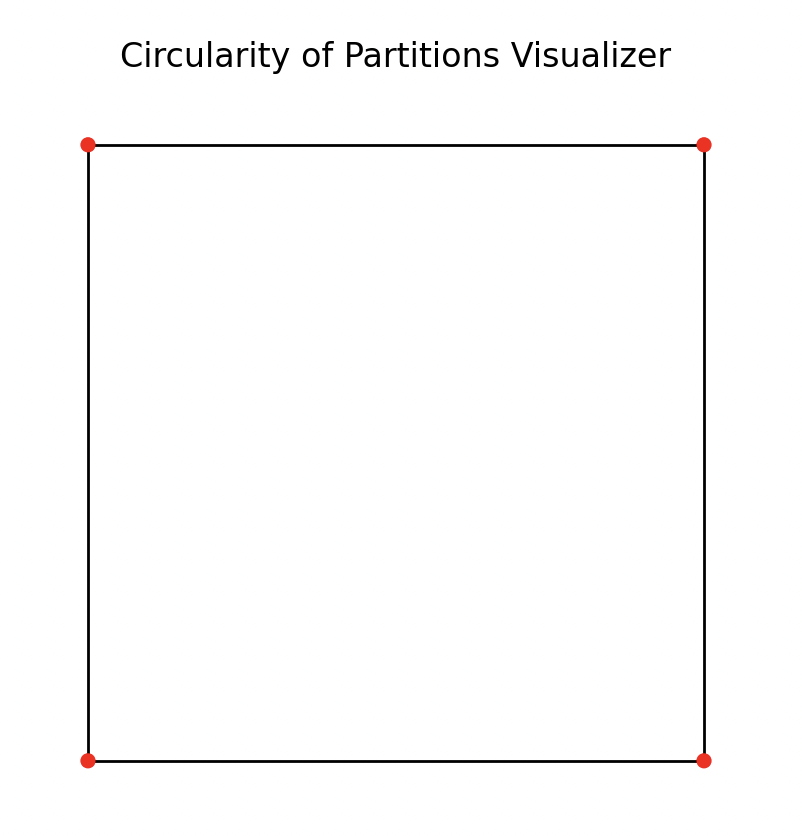
\includegraphics[scale=0.33]{SetupScreen.png} &
      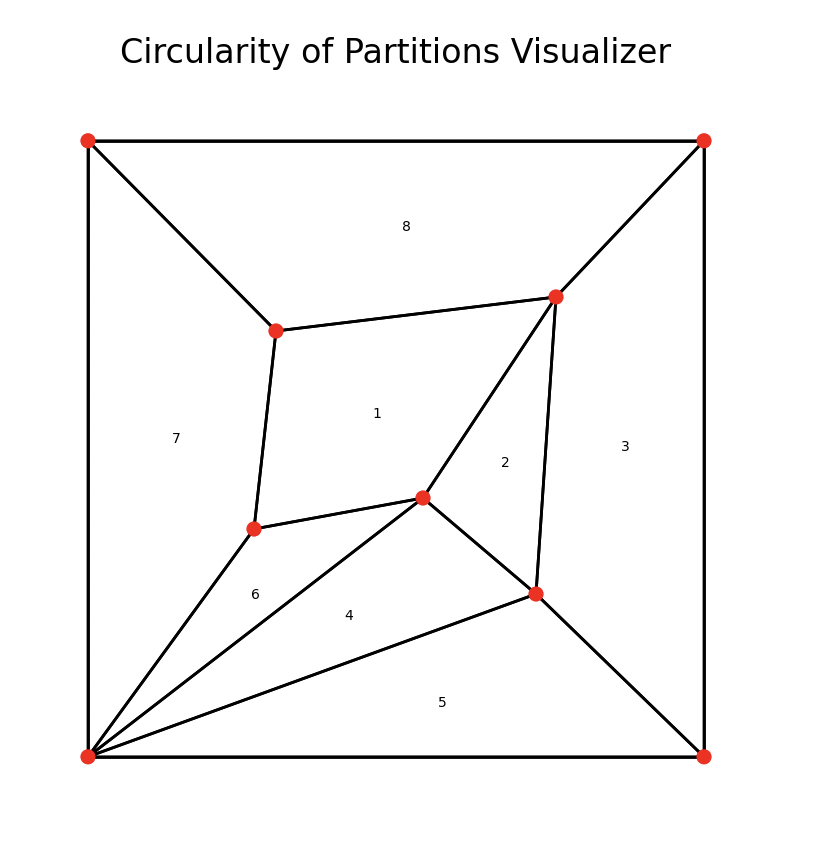
\includegraphics[scale=0.33]{UserPartition.png} &
      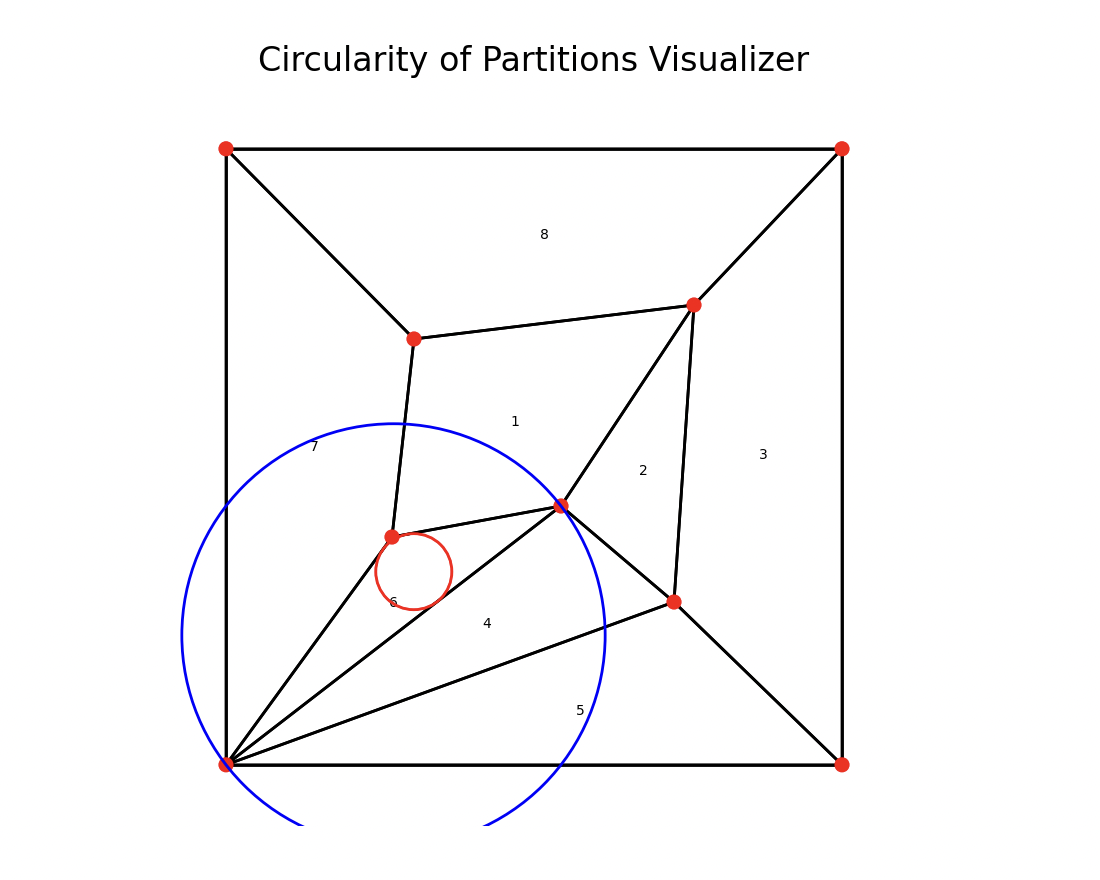
\includegraphics[scale=0.33]{CircumcircleAndIndiskOutput.png} \\
      Setup Scree (`t' key) & User-Specified Partition (`v' key) & Circumcircle and Indisk (`d' key)
    \end{tabular}
    \end{center}
    
    \begin{center}
    
\includegraphics[width=\linewidth]{CircularityOutput.png}
    \end{center}

The above process can be repeated for any user-specified partition of the square, given that all the polygonal pieces in the partition are convex. The maximum circularity
over all pieces will be calculated and printed.

\section{Future Work: Extensions}

In my visualizer, I focus on the case where the regular polygon to be partitioned is a square; this is because its optimal circularity remains to be studied \cite{damian_rourke}. 
However, I could and should extend my work to visualize any regular polygon. \\

Furthermore, there is some functionality in the visualizer that I could add and fix. I implemented an undo key to help in my debugging process, but there are aspects of the undo that remain to be completed
(for example, undoing a polygon currently does not remove its corresponding label). I would also try to add buttons to my visualizer to allow for better user interaction, rather than just printing the output to the terminal as it currently stands. \\

Finally, it may help for my visualizer to be dynamic, in the sense that it may allow for users to move the selected vertices/for the polygons to change as the user moves them. This would be an ideal piece of functionality
that will be much more difficult to implement, but could lead to stronger visualization.

\section{Conclusion}
I created an interactive visualizer where a user specifies a convex partition of the square. The program will calculate the maximum circularity over all polygonal pieces and draw the largest inscribed disk
and smallest circumscribing circle for that polygonal piece. \\

This project is part of the broader problem of finding the optimal partition (minimum circularity over all pieces) of a regular polygon, which has many applications, as specified in \cite{damian_rourke}. \\

Thank you to Professor Neil Lutz for his guidance and support, and for a great semester in CS91T: Computational Geometry.
\newpage

\begin{thebibliography}{9}
    \bibitem{topp}
    Erik D. Demaine, Joseph S. B. Mitchell, Joseph O'Rourke. \textit{The Open Problems Project}. 
    Originated from Computational Geometry Column 42. Internat. J. Comput. Geom. Appl., 11(5):573-582, 2001. Also in SIGACT News 32(3):63-72 (2001), Issue 120.

    \bibitem{damian_rourke}
    Mirela Damian and Joseph O'Rourke. \textit{Partitioning Regular Polygons into Circular Pieces I: Convex Partitions.} In Proc. 15th Canad. Conf. Comput. Geom., pages 43-46, 2003. arXiv:cs.CG/030402.    

    \bibitem{nayuki}
    Nayuki. \textit{Smallest Enclosing Circle.} \href{https://www.nayuki.io/page/smallest-enclosing-circle}{Nayuki Smallest Enclosing Circle GitHub}

    \bibitem{schuster}
    Megan Schuster (2008). \textit{The Largest Empty Circle Problem}. \href{https://www.cs.swarthmore.edu/~adanner/cs97/s08/papers/schuster.pdf}{Swarthmore College, CS97: Senior Conference, 2008}
\end{thebibliography}

\end{document}
